%%%%%%%%%%%%%%%%%%%%%%% file template.tex %%%%%%%%%%%%%%%%%%%%%%%%%
%
% This is a general template file for the LaTeX package SVJour3
% for Springer journals.          Springer Heidelberg 2010/09/16
%
% Copy it to a new file with a new name and use it as the basis
% for your article. Delete % signs as needed.
%
% This template includes a few options for different layouts and
% content for various journals. Please consult a previous issue of
% your journal as needed.
%
%%%%%%%%%%%%%%%%%%%%%%%%%%%%%%%%%%%%%%%%%%%%%%%%%%%%%%%%%%%%%%%%%%%
%
% First comes an example EPS file -- just ignore it and
% proceed on the \documentclass line
% your LaTeX will extract the file if required
\RequirePackage{fix-cm}
%
%\documentclass{svjour3}                     % onecolumn (standard format)
%\documentclass[smallcondensed]{svjour3}     % onecolumn (ditto)
%\documentclass[smallextended]{svjour3}       % onecolumn (second format)
\documentclass[twocolumn]{svjour3}          % twocolumn
%
\smartqed  % flush right qed marks, e.g. at end of proof
%
\usepackage{graphicx}
%
% \usepackage{mathptmx}      % use Times fonts if available on your TeX system
%
% insert here the call for the packages your document requires
\usepackage{url}
%\usepackage{latexsym}
% etc.
%
% please place your own definitions here and don't use \def but
% \newcommand{}{}
%
% Insert the name of "your journal" with
\journalname{Journal of Science Education and Technology}
%
\begin{document}

\title{Experiences in teaching with Jupyter, Jupyterhub, and nbgrader}
%about the article that should go on the front page should be
%placed here. General acknowledgments should be placed at the end of the article.}
% \subtitle{Do you have a subtitle?\\ If so, write it here}

%\titlerunning{Short form of title}        % if too long for running head

\author{Marcin Kostur \and
        Marina Appiou-Nikiforou \and
        Andreas Papadopoulos \and
	Gert-Ludwig Ingold
}

%\authorrunning{Short form of author list} % if too long for running head

\institute{Marcin Kostur \at
              first address \\
              Tel.: +123-45-678910\\
              Fax: +123-45-678910\\
              \email{marcin.kostur@us.edu.pl}           %  \\
%             \emph{Present address:} of F. Author  %  if needed
           \and
           Marina Appiou-Nikiforou \at
              European University Cyprus, 
	      6 Diogenous Street, 1516 Nicosia, Cyprus\\
              \email{M.Nikiforou@euc.ac.cy}
	   \and
	   Andreas Papadopoulos \at
              European University Cyprus, 
	      6 Diogenous Street, 1516 Nicosia, Cyprus \\
              \email{apapado89@gmail.com}
	     % \emph{Present address:}
	   \and
	   Gert-Ludwig Ingold \at
	      Institut f{\"u}r Physik, Universit{\"a}t Augsburg,
	      Universit{\"a}tsstra{\ss}e 1, 86135 Augsburg, Germany\\
	      \email{gert.ingold@physik.uni-augsburg.de}
}

\date{Received: date / Accepted: date}
% The correct dates will be entered by the editor


\maketitle

\begin{abstract}
Insert your abstract here. Include keywords, PACS and mathematical
subject classification numbers as needed.
\keywords{First keyword \and Second keyword \and More}
% \PACS{PACS code1 \and PACS code2 \and more}
% \subclass{MSC code1 \and MSC code2 \and more}
\end{abstract}

\section{Introduction}
\label{intro}

Using technology in everyday teaching is something that we, as instructors, 
should all consider. Using technology for educational purposes is the key to moderate 
the gap between students of the new era, students who are being brought up and with 
technology, and us the instructors of the old era, who were brought up with no internet 
available and are trying to catch up with technology. 
 
In recent years, Python has become increasingly popular as a first programming
language at universities. Due to its expressive code, it provides a low entry
barrier for students while at the same time being well suited for serious
scientific work (for prominent recent examples see \cite{gw150914} and
\cite{EHT}). In a teaching environment, the availability of a Python
distribution for all operating systems likely to be used by students proves to
be very helpful to ensure a consistent working environment for all students.

 
The development of the Jupyter notebook has opened up exciting new
possibilities in teaching \cite{jupyter-edu-book}. At the same time,
the Jupyter notebook has become the de facto standard among data
scientists. Employing the Jupyter notebook in teaching provides the
students not only with new way to learn but also with a tool potentially
useful for their further career.

While it is possible to run the Jupyter notebook with a Python kernel on the
students' computer, the fact that work with the Jupyter notebook is browser-based
suggests to provide students with an access to a Python kernel via a Jupyterhub.
This approach avoids any installation requirements on the students' side besides
the availablility of a browser.

For the Jupyter notebook, the extension \texttt{nbgrader} was developed
\cite{nbgrader} which serves as a tool to distribute, collect and grade problem
sets for exercises. In the most recent version (0.6.0) at the time of this
writing, the possibility of giving feedback to students has been significantly
facilitated.


\section{Introduction new technologies in teaching in mutual collaboraion}


Back in 2017 the collaboration between three partners University of
Augsburg, European University Cyprus and University of Silesia has
been initiated in the form of Erasmus+ project. The general aim was to
research on possibility of implementing good practices in using Python
programming language and Jupyter notebook in teaching in different
environments. Experience among parters with both Python and Jupyter
were diversified. It opened a possibility to observe a process of an
adoption of new educatioal approach at different phases at the same
time.

The collaboration consisted on three elements: creation of software
infrastructure, authoring course materials and experimenting with
elements of Test Driven Development process using nbgrader.


\subsection{University of Aubgsburg} 

At the university of Augsburg, programming courses for students of physics and
materials science are offered since about ten years. During that time, the
exercises mentioned in \label{sec:nbgrader} have been gradually developed and
tested in exercise sessions organized in groups of two or three students under
guidance of teaching personnel. This format was also be used to develop the
Jupyter notebooks. The close interaction between students and teachers allowed
to analyze the way students make use of the notebooks and to identify problems
in the tests used to do the grading and to improve these tests. While the courses
so far had about 10-20 students, we expect to have of the order of 100 students
from next year on. Then, the experience collected with \texttt{nbgrader} will
be very valuable.

In the lectures on programming, Jupyter notebook have succesfully been used for
several years for teaching. In addition, students were encouraged to use them
during the lectures on their laptop but were found to rarely make use of this
opportunity. They mostly preferred to attentively follow the lecture. However,
Jupyter notebooks were offered to students for download so that they could
work on them at home. It is not clear, how much use was made of this possibility.
On the other hand, in the regular physics courses, Jupyter notebooks have been
rarely used and probably will not be used for an entire course. However, we
expect to use Jupyter notebooks more often for demonstration purposes where
appropriate.

\subsection{University of Silesia}

At the University of Silesia Python used to be a a first programming
language for students of Applied Computer Science. There has beem
implemented a concept of ``mobile computer classroom'' which consists
of inexpensive and mobile computers which are are available to
students in the rental office. Initially it consisted of 10-inch
netbooks, currently the hardware is based on Chromebooks which are
very easy to maintain. Therefore an important aspect is the
accessibility of the work environment in a web browser. Jupyter
notebook fits perfectly in such a scenario. In recent years several
work scenarios based on Juyter notebook have been developed in such an
environment.

Here, we will mainly concentrate on the case of course ``Introduction
to Artifitial Intelligence``, which is attented by c.a. 50 students
every year. The course used Jupyter notebook as a teaching tool during
the lectures and tutorials. Students had to submit their work in the
form of notebooks form. Additionally automating testing software has been 
used to help both students as well as teachers.


\subsection{University of Cyprus}





\section{Jupyter and Jupyterhub}
\label{sec:jupyter_jupyterhub}

Generally speaking, a Jupyter notebook is a document mixing prose,
code, visualization, together with resources: source code, data,
media.  It consists of a collection of two types of cells, namely code
cells and text cells (see fig. \ref{fig:notebook}). The latter may
contain text written in markdown, possibly including formulas as well
as figures. This structure facilitates to guide students through a
problem set.

\begin{figure}
  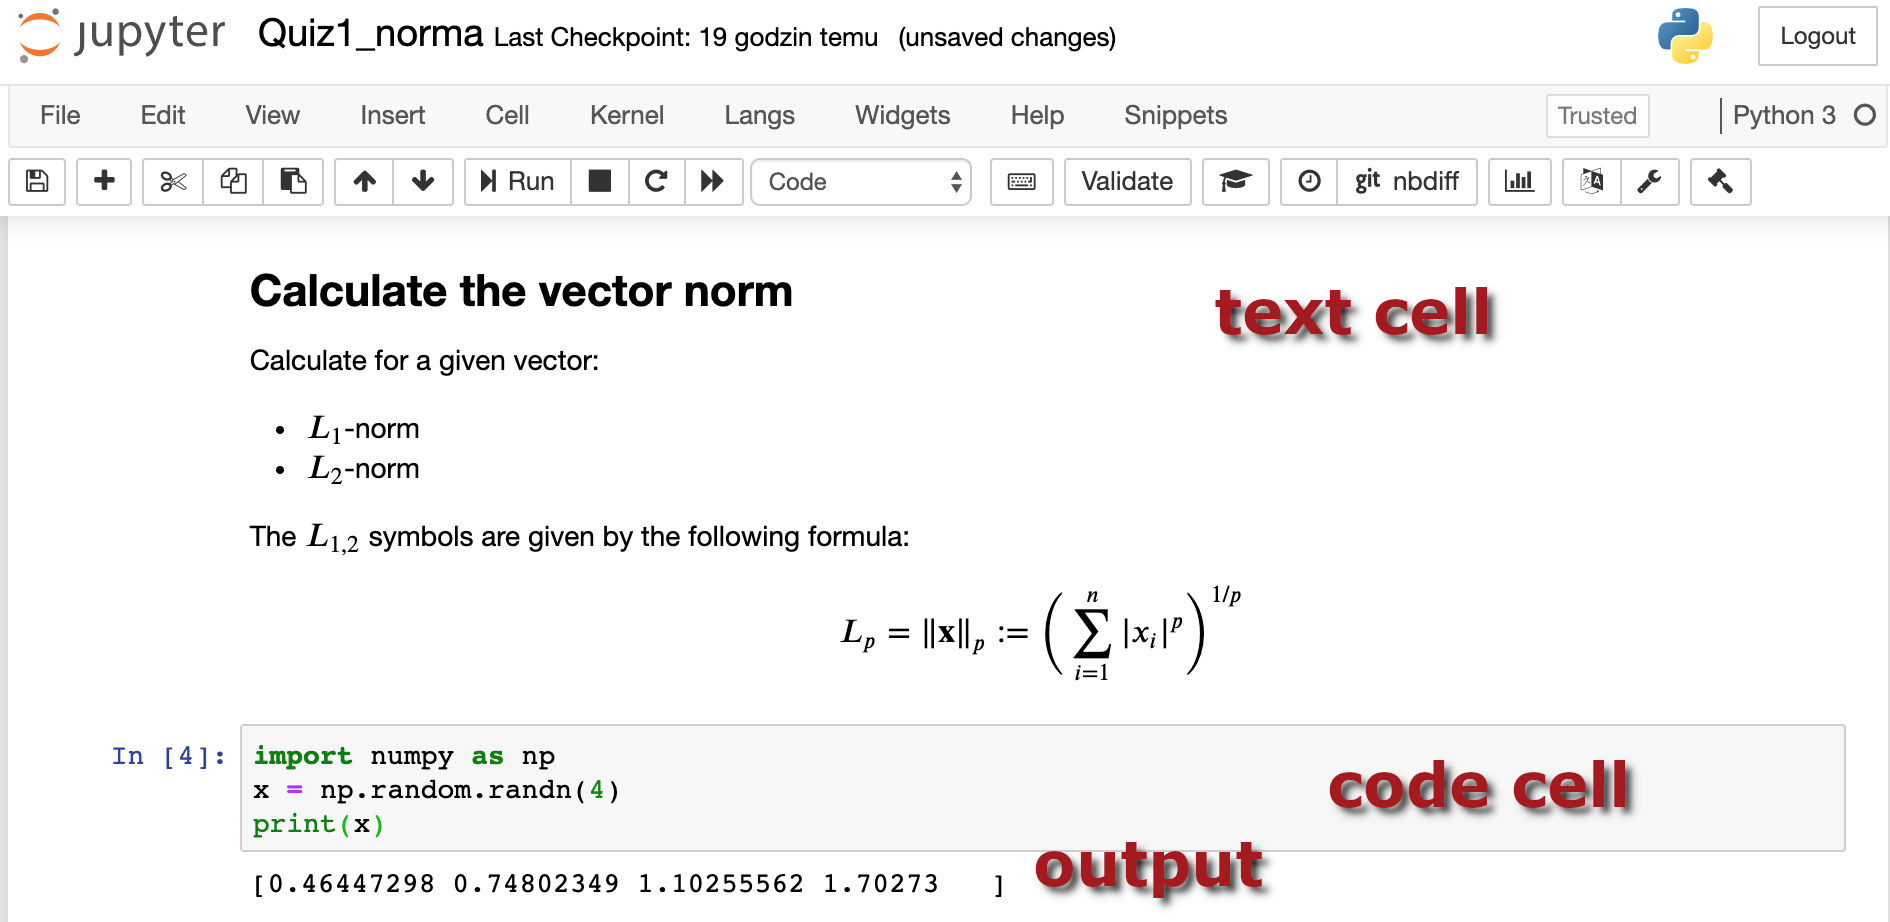
\includegraphics[width=0.5\textwidth]{figs/notebook.png}
\caption{Jupyter notebooks is a executable document which contains
  rich-text and code (e.g. in Pyton). }
\label{fig:notebook}
\end{figure}

Jupyter notebook has recenely been popular among researchers as it can
embody the FAIR (Findable, Accessible, Interoperable, Reusable)
principles for scholarly communication \cite{Randles2017}. The number
of notebooks which are publically available on github now exceeds 5
milion.


Jupyterhub a software providing a way to serve Jupyter notebook for
multiple users. It can be used in a classes of students, all

 a centrally provided resource to run a Jupyter notebook from a
remote computer makes problem sets or more generally teaching material easily
accessible without the need for a local Python installation. Furthermore, this
approach ensures a consistent working environment for all students. However,
it might be an important experience for students that all work which they
are doing could in fact be done on their own computer instead of using some
remote service where the underlying machinery is completely hidden.

\section{\texttt{nbgrader}}

\subsection{Functions}

In \texttt{nbgrader}, the solutions should be implemented in terms of a
function, so that this function can be tested, typically for different
parameters. As a consequence, the concept of functions needs to be introduced
early on in a course. However, the use of functions will be close to the
concept of a mathematical function in the sense that there will be input values
and output values. In the tests used to grade the answer, one wants to vary the
input values and the output value is the object which is to be tested against
an expectation. Therefore, situations like the absence of arguments or return
values as well as default arguments and keyword arguments representing more
advanced concepts, are not required to work with \texttt{nbgrader}.

It is good programming practice to logically structure code into functions of a
not too large length. Students with \texttt{nbgrader} thus get used to this
practice early on, in particular if functions are used to build up the final
solution step by step. The drawback however is that this structure is provided
to them by the teacher. Students are not actively structuring their code by
themselves and thus do not really exercise this practise.

In Python, the use of docstrings is highly recommended as way to document
the behavior of a function. For the use with \texttt{nbgrader}, teachers are
naturally using docstring because they need to specify the purpose of the
function and the meaning of the input and output values. Students will thus
soon consider docstring as standard part of a function. However, they do not
actively practice the habit of annotating a function with a docstring.

The version of a function released to the students by \texttt{nbgrader} by
default raises a \texttt{NotImplementedError}. This statement ensures the
correct working of the function during grading even if no solution is provided.
Students need to remove the statement and replace it by their solution. It was
found both in the German as well as the Polish group of students that this need
was somewhat difficult to convey to them. This difficulty likely arises from
the fact that students have not been taught the meaning of the \texttt{raise}
statement. They therefore need to be especially alerted to what they need to do
with this statement and internalize the removal of the \texttt{raise} statement
as a recipe.

\subsection{Grading with tests}

The main idea for autograding with \texttt{nbgrader} consists in the teacher
providing one or several tests while the student needs to develop code which
satisfies theses tests. This strategy is typical for test-driven development,
a component of agile programming where tests are written before the code.
The use of \texttt{nbgrader} thus offers an opportunity to discuss the role
of testing and the concept of test-driven development. However, it certainly
depends on the programming background of the specific students whether such
remarks are fruitful. While one should not expect that students get into the
habit of test-driven development right away, the concept might stick in their
mind and be activated at a later time.

The experience in both, the German and the Polish groups was that tests in
\texttt{nbgrader} problem sets should not only pertain to the specific
functionality of a solution to be developed by the student. It turned out
that mistakes like not returning a result or returning a result of an incorrect
type do not only occur when students start working with \texttt{nbgrader} but
also in later stages. It has therefore proven useful to separate tests into
two groups. The first groups of tests check for the existence of a result
and for the correct type. These are prerequisites for the second group of results
which test the functionality of the proposed solution for correctness.

The first group of tests should mainly be considered as an opportunity to
provide feedback to the students. They could be alerted to a missing return
value by the test

\noindent\texttt{assert result is not None, 'Does your function return
a result?'}

Quite generally, tests in \texttt{nbgrader} should not only be considered as
tool for grading but also as an opportunity to give helpful feedback to the
students while working on the problem set. Providing an expressive error
message will be helpful for many students who are not yet capable to understand
or correctly interpret the standard traceback of a Python exception. 

A problem very frequently encountered with students results from detailed 
tests with clear error messages. Students were found to rely in their assessment
of correctness of their solution almost entirely on the results of the tests.
In other words, they typically do not develop a critical attitude towards their
code and do not see the need of doing their own tests. One could imagine to
have several blocks of tests to demonstrate that the passing of a number of
tests does not necessarily need that the code is correct. Setting up such a
test suite however relies on a good knowledge of typical mistakes which can
be exploited.

\subsection{Addressing heterogeneity}

It is not uncommon that in programming courses one has to address an audience
with a wide range of programming capabilities. Some students have no
programming experience whatsoever and might even show a code writing block
while others have an extensive programming experience, often in a different
programming language. For students with little or no programming experience,
more complex exercise problems need to be decomposed into a number steps while
experienced students might tackle the problems directly without any additional
help. The latter students often are proficient in a language different from
Python. A typical indicator are loops over indiced instead of objects contained
in a list. Here, the feedback mechanism of \texttt{nbgrader} comes handy, in
particular for \texttt{nbgrader} version 0.6+.

At the same time, the solution of the problem should provide a source of
satisfaction for all students. When teaching programming to science students, a
way could be to appeal to the respective scientific background. However, such
problem sets are often experienced as an unnecessary mental burden.

In exercise work with \texttt{nbgrader}, we have experimented with allowing for
individual learning paths by providing one main Jupyter notebook and typically
a few subnotebooks. The main notebook provides the problem description and the
notebook cells where the final solution should be developed. The subnotebooks
focus on one aspect of the solution so that students can work towards a complete
solution step by step.

To illustrate our approach by way of an example, we consider a problem set
where a graphical representation of a Julia set shall be generated. Students
need to repetitively carry out an interation $z\rightarrow z^2+c$ where $c$ is
a given complex constant and the iteration starts from complex values $z_0$
taken on a grid in the complex plane. The Julia set distinguishes between the
initial conditions for which $z$ converges from those where $z$ remains bounded.
In practice, this distinction can be achieved by checking whether an appropriately
chosen bound is crossed within a given maximum number of iterations. A beautiful
graphical representation can be obtained by converting the number of iterations
actually needed to cross the bound into a color. 

This problem presents a number of difficulties to the students. From an
algorithmic point of view, the iteration needs to be implemented and stopped
once either the bound is crossed or the maximum number of iterations has been
reached. On a more conceptual level, students were often found to encounter
problems in imagining how a computer can represent colors. A subnotebook
explaining the concept of a colormap and allowing students to explore the
translation of a number into a color representation turns out to be helpful.
Here, the rich output of the Jupyter notebook is used by providing a SVG
representation of a square filled with the respective color. Care needs to
be taken that the students are not irritated by the code needed to provide
the infrastructure for generating the colored square. The opportunity of
playing with the conversion of a number into a visual representation of a
color usually turns out to be very helpful. At this point, a background of
the RGB or HSV representation of colors is not necessarily required but
can be offered to interested students in a separate subnotebook.

Another conceptual obstacle for beginners is the idea of pixels in an image
and how to walk along a two-dimensional grid or even a one-dimensional grid
within a program. This aspect thus deserves a separate subnotebook and proceeding
in steps from one to two dimensions proved to be useful. The main reason for
addressing the one-dimensional case first is due to the observation that if
students are asked to produce a given number of equally spaced points between
two values, they typically confuse the number of points with the number of
intervalls between the points. This issue needs to be first clarified in one
dimension before the two-dimensional case can be addressed.

Structuring a problem into a number of steps with their own notebooks allows to
offer individual learning paths. In the supervised exercise sessions it turned
out that the vast majority of students tends to follow the step-by-step
learning path which led most directly to the solution. In other words, students
would have needed very strong encouragement to try to develop the solution
completely on their own. On the other hand, students typically did not go through
the additional material provided on the RGB and HSV representation.

On a more technical level, it could be observed that the fact that opening a
new notebook would lead to an extra tab in the browser could become quite
confusing for the students unless the take care to close tabs not needed
anymore. In particular, it happened that the students opened notebooks more
than once and then getting confused in which notebook they were actually
working.

Using \texttt{nbgrader} in a scenario as described above, an additional
difficulty arises in the grading. Students working on subnotebooks should earn
the respective points even if they are able to only solve some of the steps
successfully. On the other hand, a student who solves the problem without going
through all the notebooks should not be punished. The \texttt{nbgrader}
database holds all the points obtained for the various notebooks, from which a
final number of points can be determined. This is however a functionality not
directly provided by \texttt{nbgrader}. If points are assigned appropriately to
the individual tasks, one can determine the number of points earned as the
minimum of the total sum of points earned and the maximum number of points
attributed to the problem set.


\section{Problems and pitfalls in using Jupyter notebook}
Usually, the code in a notebook is intended to be executed in a linear
fashion even though this is not imposed by the notebook. In fact, the
notebook should invite students to experiment which implies the
opening of new cells and the execution of code written by the
student. In this process, out-of-order execution naturally occurs and
can have side effects which tend to confuse students. While the order
of execution of individual cells can be inferred by the sequence
number attributed to a cell once it has been executed, in particular
beginners are not aware of the problems that out-of-order execution
can entail.


Using the Jupyter notebook for exercises is interesting because
students can easily experiment with code. At the same time one should
be aware that students might think that this is the standard way of
programming in Python. While it is indeed possible to develop pieces
of a more complex program in the Jupyter notebook and later combine
these pieces, this is not the standard approach for complex
programming tasks. Therefore, students should also be acquainted with
the IDEs like Spyder distributed with the Anaconda distribution or the
use of editors like vim or others which can be configures to support
programming in Python.


\section{Conclusion}





\begin{acknowledgements}
This work was supported by the European Union through Erasmus+ project
2017-1-PL01-KA203-038747.
\end{acknowledgements}

\section*{Conflict of interest}
The authors declare that they have no conflict of interest.


%% For one-column wide figures use
%\begin{figure}
%% Use the relevant command to insert your figure file.
%% For example, with the graphicx package use
%  \includegraphics{example.eps}
%% figure caption is below the figure
%\caption{Please write your figure caption here}
%\label{fig:1}       % Give a unique label
%\end{figure}
%%
%% For two-column wide figures use
%\begin{figure*}
%% Use the relevant command to insert your figure file.
%% For example, with the graphicx package use
%  \includegraphics[width=0.75\textwidth]{example.eps}
%% figure caption is below the figure
%\caption{Please write your figure caption here}
%\label{fig:2}       % Give a unique label
%\end{figure*}
%%
%% For tables use
%\begin{table}
%% table caption is above the table
%\caption{Please write your table caption here}
%\label{tab:1}       % Give a unique label
%% For LaTeX tables use
%\begin{tabular}{lll}
%\hline\noalign{\smallskip}
%first & second & third  \\
%\noalign{\smallskip}\hline\noalign{\smallskip}
%number & number & number \\
%number & number & number \\
%\noalign{\smallskip}\hline
%\end{tabular}
%\end{table}



% BibTeX users please use one of
%\bibliographystyle{spbasic}      % basic style, author-year citations
%\bibliographystyle{spmpsci}      % mathematics and physical sciences
%\bibliographystyle{spphys}       % APS-like style for physics
%\bibliography{}   % name your BibTeX data base

% Non-BibTeX users please use
\begin{thebibliography}{99}
%
% and use \bibitem to create references. Consult the Instructions
% for authors for reference list style.
%
\bibitem{gw150914}
% https://doi.org/10.1103/PhysRevD.93.122003
Abbott, B. P. \textit{et al.} (2016).
GW150914: First results from the search for binary black hole coalescence with Advanced LIGO,
\textit{Physical Review D}, 93(12), 122003.

\bibitem{Randles2017}
B. M. {Randles} and I. V. {Pasquetto} and M. S. {Golshan} and C. L. {Borgman}
2017 ACM/IEEE Joint Conference on Digital Libraries (JCDL),
2017, doi={10.1109/JCDL.2017.7991618}

\bibitem{EHT}
% https://doi.org/10.3847/2041-8213/ab0c57
The Event Horizon Telescope Collaboration (2019).
First M87 Event Horizon Telescope Results. III. Data Processing and Calibration,
\textit{The Astrophysical Journal Letters} 875(1), L3.

\bibitem{jupyter-edu-book}
Barba, L. A., Barker, L. J., Blank, D. S., Brown, J, Downey, A. B., George, T.,
Heagy, L. J., Mandli, K. T., Moore, J. K., Lippert, D., Niemeyer, K. E.,
Watkins, R. R., West, R. H., Wickes, E., Willing, C., \& Zingale M. (2019).
Teaching and Learning with Jupyter,
\url{https://jupyter4edu.github.io/jupyter-edu-book/}.

\bibitem{nbgrader}
% https://doi.org/10.21105/jose.00032 
Project Jupyter, Blank, D., Bourgin, D., Brown, A., Bussonnier, M.,
Frederic, J., Granger, B., Griffiths, T. L.,  Hamrick, J., Kelley, K.,
Pacer, M., Page, L., P{\'e}rez, F., Ragan-Kelley, B., Suchow, J. W.,
\& Willing, C. (2019).
nbgrader: A Tool for Creating and Grading Assignments in the Jupyter Notebook,
\textit{Journal of Open Source Education}, 2(11), 32.
% Format for books
%\bibitem{RefB}
%Author, Book title, page numbers. Publisher, place (year)
% etc
\end{thebibliography}

\end{document}
